\documentclass[12pt,a4paper]{article}
\usepackage{microtype}
\usepackage{lmodern}
\usepackage{mathpazo}
\usepackage{latexsym}
\usepackage{amsmath,amssymb,amsthm}
\usepackage[english]{babel}
\usepackage{float}
\usepackage{graphicx}
\usepackage{subcaption}
\usepackage{hyperref}
\usepackage[utf8]{inputenc}
\usepackage{listings}
\usepackage{xcolor}
\usepackage{colortbl}
\usepackage{enumitem}
\usepackage{multirow}
\usepackage{tabularx}
% use more of the page
\usepackage[scale=0.8]{geometry}
% do not move figures across sections
\usepackage[section]{placeins}

% Sensible defaults for lstlistings
\lstset{
  basicstyle=\footnotesize\ttfamily,
  belowcaptionskip=1\baselineskip,
  breaklines=true,
  commentstyle=\bfseries\color{purple!40!black}
  frame=L,
  identifierstyle=\color{blue},
  keywordstyle=\bfseries\color{green!40!black},
  language=python,
  showstringspaces=false,
  stringstyle=\color{orange},
  xleftmargin=\parindent,
}
% prettier links
\hypersetup{
colorlinks,
linkcolor={red!50!black},
citecolor={blue!50!black},
urlcolor={blue!80!black}
}
\urlstyle{rm}

\begin{document}
\title{Advanced Deep Learning\\Assignment 3}
\author{Johannes Sindlinger, Christoph Kern, Amos Weckström}
\maketitle

\tableofcontents

\newpage




\section{Part B. Recurrent Neural Networks}

\subsection{Task \& Data}

In this task, we evaluated RNNs and LSTMs on recognizing sequences of the form \(a^nb^nc^n\). Training data comprised sequences ranging from 1 to 20 characters, while testing sequences spanned 21 to 100 characters. The dataset included two types of sequences:
\begin{enumerate}
    \item Real Sequences (True Labels): These sequences were of the form \(a^kb^kc^k\), where \(k\) was a randomly drawn number between \(\text{min\_length}/3\) and \(\text{max\_length}/3\). We generated half of the dataset using these real sequences. Though some duplicates were inevitable due to the limited number of true labels, for the test set, we removed duplicates.
    \item The remaining half of the dataset consisted of sequences not belonging to the formal language. These sequences were generated using two methods:
    \begin{itemize}
        \item Random Sampling: This method constituted 70\% of the false examples. Numbers \(k\), \(m\), and \(n\) were randomly generated, subject to the condition \(\text{min\_length} \leq k+m+n \leq \text{max\_length}\), and a sequence \(a^kb^mc^n\) was created. We ensured that these sequences did not accidentally belong to the formal language.
        \item Noise Sampling: This method constituted 30\% of the false examples. Real sequences were randomly created as described above, and then a character was randomly added or deleted to introduce noise.
    \end{itemize}
\end{enumerate}

\subsection{Predictive Models}
We implemented the two models using the PyTorch RNN and LSTM modules:
The data is entered as a one-hot-encoded vector / embedding for the three different characters and then passed to the RNN-/LSTM-module. The last output of the RNN-/LSTM-module is then passed on towards a final linear layer with sigmoid activation. The size of the hidden layers of the RNN-/LSTM-neurons and the amount of layers in the RNN-/LSTM-module are part of the cross-validation of the hyperparameter search.
\subsection{Experimental Setup}
To compare the two models, we constructed a dataset with $N=2000$ training samples, each with a sequence length ranging from 1 to 21. We kept the data set size small in order to limit the computing time. However, this limits the informative value of the results. For the test dataset, we followed the same procedure and generated $N=500$ samples with sequence lengths ranging from 20 to 200. In the test data set, duplicates were removed. Therefore, the test data set is not balanced. \textbf{The average sequence length of the test data was 60.3.}

Both models were trained using a cross-validation approach to determine the optimal parameter combinations for each. We evaluated the performance of the models using the following parameter combinations:
\begin{center}
    \begin{tabular}{|c|c|c|}
\hline
Hidden Layer Size & Learning Rates & Number of RNN/LSTM-Layers \\
\hline
4, 8, 16 & 0.01, 0.001 & 1, 2 \\
\hline
\end{tabular}
\end{center}

We trained each model for \textbf{10 epochs} using \textbf{Adam optimizer} and \textbf{Binary Cross Entropy loss}. \textbf{For the evaluation we used F1-score as the data set is not balanced as explained earlier}.
\subsection{Results \& Discussion}
The following table shows the top 4 results for both models: \\

\scriptsize
\noindent
\begin{minipage}[c]{0.5\textwidth}
\[
\begin{array}{|c|c|c|c|}
\hline
\text{Hidden size} & \text{Learning rate} & \text{Num layers} & \text{F1 score} \\
\hline
8 & 0.01 & 2 & 0.6585 \\
4 & 0.01 & 2 & 0.4779 \\
16 & 0.001 & 2 & 0.4583 \\
4 & 0.001 & 1 & 0.4463 \\
\hline
\end{array}
\]
\begin{center}
    \textbf{(a) RNN}
\end{center}
\end{minipage}\hfill
\begin{minipage}[c]{0.5\textwidth}
\[
\begin{array}{|c|c|c|c|}
\hline
\text{Hidden size} & \text{Learning rate} & \text{Num layers} & \text{F1 score} \\
\hline
16 & 0.01 & 2 & 0.9818 \\
16 & 0.01 & 1 & 0.7119 \\
4 & 0.01 & 2 & 0.4954 \\
8 & 0.01 & 1 & 0.4381 \\
\hline
\end{array}
\]
\begin{center}
    \textbf{(b) LSTM}
\end{center}
\end{minipage}\vspace{0.5em}

\normalsize

The following figure \ref{fig:test} displays the top-performing results of the RNN and LSTM models, with F1-scores calculated across sequence lengths incremented by 10 steps.

\begin{figure}[!htb]
\centering
\begin{subfigure}{.5\textwidth}
  \centering
  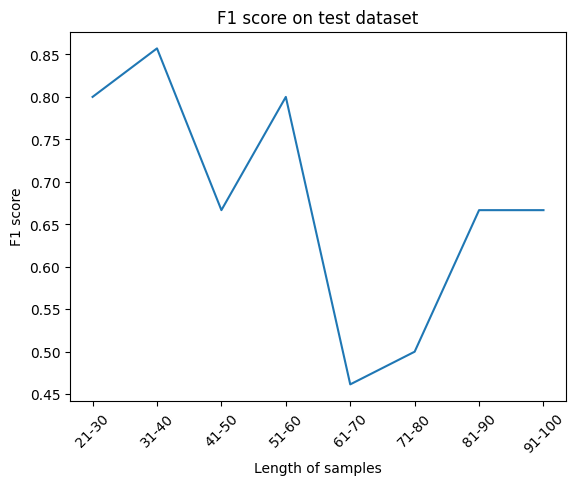
\includegraphics[width=.6\linewidth]{Assignment_3/Report/Figures/rnn.png}
  \caption{RNN}
  \label{fig:sub1}
\end{subfigure}%
\begin{subfigure}{.5\textwidth}
  \centering
  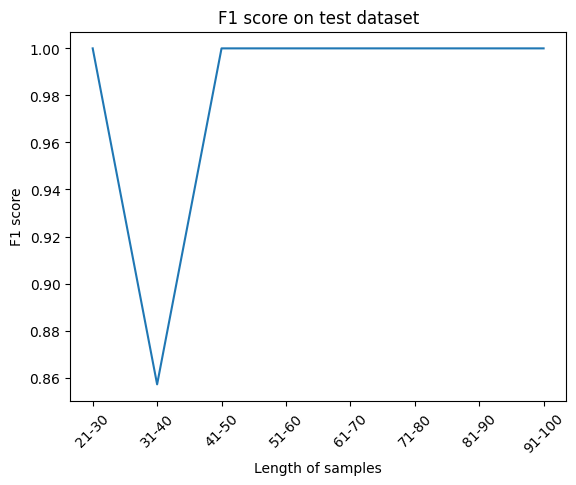
\includegraphics[width=.6\linewidth]{Assignment_3/Report/Figures/lstm.png}
  \caption{LSTM}
  \label{fig:sub2}
\end{subfigure}
\caption{F1-score for sequence buckets of 10 of the top-performing combinations of parameters.}
\label{fig:test}
\end{figure}

The \textbf{LSTM exhibits the highest F1-scores}, indicating its superiority over the RNN model. Optimal performance is attained by the LSTM model featuring a hidden size of 16, a learning rate of 0.01 and the usage of 2 LSTM-layers. Conversely, the RNN model demonstrates no discernible pattern in parameter selection. Nonetheless, the utilization of two layers within the RNN-module consistently appears within the top three results.

Figure \ref{fig:test} illustrates a \textbf{notable decline in performance of the RNN model as sequence length increases, whereas the LSTM maintains consistent accuracy}, with only one deviation observed in the 31-40 range. This observation aligns with the inherent design of the two networks, wherein LSTMs, equipped with various gates, are specifically engineered to effectively retain information from longer sequences.

\subsection{Conclusion}

According to the analysis provided, it is evident that LSTMs outperform Vanilla RNNs in their capacity to retain information from longer sequences and in performing classification tasks. However, it is noteworthy that among the 12 models tested, only one achieves highly reliable classification with an F1-score surpassing 0.9. This indicates that while LSTMs offer advantages, they are not universally applicable solutions for all scenarios.

\newpage





\section{Part C. Zero-shot Prompting}

\subsection{Task \& Data}

In this task, we will test the zero-shot performance on two LLMs by letting them predict whether the following two tweets are from a real or parody account.\vspace{0.5em}

\footnotesize
\noindent
\begin{minipage}[c]{0.37\textwidth}
    \textbf{Tweet 1 (real):}
    \emph{It’s the \#GimmeFive challenge, presidential style.}
\end{minipage}\hfill
\begin{minipage}[c]{0.6\textwidth}
    \textbf{Tweet 2 (parody):}
    \emph{It’s up to you, America, do you want a repeat of the last four years, or four years staggeringly worse than the last four years?}
\end{minipage}\vspace{0.5em}

\normalsize

\noindent We will use two different prompts: one phrased as a question, one phrased as an instruction.\vspace{-0.5em}


\subsection{Experimental Setup}

Following initial prompts were considered. By doing some rudimentary testing on each template with the given tweets using ChatGPT 3.5 and looking at the quality and consistency of the results, we chose one template for each type.\vspace{0.5em}

\noindent
\begin{minipage}[c]{0.53\textwidth}
\textbf{Question types:}\vspace{-0.3em}
\scriptsize
\begin{enumerate}[itemsep=1pt, left=0pt]
    \item \texttt{Is the tweet "\textcolor{blue}{\{tweet\}}" from a real politician or parody account? Answer the question with either "real" or "parody".}
    % Is the tweet "{tweet}" from a real politician or parody account? Answer the question with either "real" or "parody".

    % llama 70B answered "parody"
    
    \item \texttt{Consider following tweet: "\textcolor{blue}{\{tweet\}}". Can you identify if it is from a parody account or a real politician account? Answer with "real" or "parody" only!}
    % Consider following tweet: "{tweet}". Can you identify if it is from a parody account or a real politician account? Answer with "real" or "parody" only!

     % llama 70B answered "parody"

    \item \texttt{Is the following tweet from a real politician account or a parody account? Tweet: "\textcolor{blue}{\{tweet\}}". Do not elaborate on the answer, just respond with "real" and "parody".} \label{prompt:q_3}
    % Is the following tweet from a real politician account or a parody account. Tweet: "{tweet}". Do not elaborate on the answer, just respond with "real" and "parody".
    
\end{enumerate}
\vspace{-1em}
\normalsize

Chosen as \textbf{Template A}: prompt \ref{prompt:q_3} 
\end{minipage}\hfill
\begin{minipage}[c]{0.46\textwidth}
\textbf{Instruction types:}\vspace{-0.3em}
\scriptsize
\begin{enumerate}[itemsep=1pt, left=0pt]
    \item \texttt{Please determine whether the following tweet is from a real politician or a parody account: "\textcolor{blue}{\{tweet\}}". Reply only with "real" or "parody".}
    % Please determine whether the following tweet is from a real politician or a parody account: "{tweet}". Reply with "real" or "parody".

    % llama 70B answered "real"
    
    \item \texttt{Decide if this tweet is from a real politician or a parody account: "\textcolor{blue}{\{tweet\}}". Only answer with "real" or "parody".}
    % Decide if this tweet is from a real politician or a parody account: "{tweet}". Answer with "real" or "parody".

    % llama 70B answered "real"

    \item \texttt{Classify the following tweet as being from a real politician account or a parody account: "\textcolor{blue}{\{tweet\}}". Respond with "real" or "parody" only.} \label{prompt:i_3}
    % Classify the following tweet as being from a real politician account or a parody account: "{tweet}". Respond with "real" or "parody" only.

    % llama 70B answered "real"
\end{enumerate}
\vspace{-2em}
\normalsize

Chosen as \textbf{Template B}: prompt \ref{prompt:i_3}
\end{minipage}
\vspace{-0.3em}

\subsection{Evaluation}

We chose following two models to battle in the Chatbot Arena: \vspace{-0.3em}
\footnotesize
\begin{center}
\begin{tabular}{ m{1.6cm} | m{1.9cm}  m{2.1cm}  m{2cm}  m{7cm} }
\textbf{Model} & \textbf{Parameters} & \textbf{Open Source} & \textbf{Developer} & \textbf{Architecture Type} \\ 
\hline
\texttt{llama-70b} & 70 billion & Yes & Meta & Optimized transformer with Grouped-Query Attention (GQA) \\ 
\hline
\texttt{command-r} \texttt{-plus} & 104 billion & Partially & Cohere & Transformer with advanced tool use and retrieval-augmented generation (RAG) \\ 
\end{tabular}
\end{center}
\normalsize
\vspace{-0.6em}

\subsection{Results \& Analysis}

The results can be seen in Figures \ref{fig:A1}, \ref{fig:B1}, \ref{fig:A2}, and \ref{fig:B2}, and are summarized in following table:\vspace{-0.3em}

\footnotesize
\begin{center}
\begin{tabular}{c c | c c c}
 \textbf{Tweet} & \textbf{Template} & \texttt{llama-70b} & \texttt{command-r-plus} & \textbf{True Label} \\ \hline
\multirow{2}{*}{1} & A & Real & \textcolor{red}{Parody} & \multirow{2}{*}{Real}  \\
 & B & Real & \textcolor{red}{Parody} \\ \hline
\multirow{2}{*}{2} & A & Parody & Parody & \multirow{2}{*}{Parody} \\
 & B & Parody & \textcolor{red}{Real} & \\
\end{tabular}
\end{center}
\normalsize
\vspace{-0.4em}

\noindent We observe that \texttt{llama-70b} consistently identified the real and parody tweets correctly across both templates, indicating a robust zero-shot performance for this task. A possible cause for this great performance might be that these exact tweets are contained in its training set. On the other hand, \texttt{command-r-plus} only correctly identified the Tweet 2 for Template A. %, it mislabeled Tweet 1 for both templates and Tweet 2 for Template B. 
This suggests that to a certain degree the classification ability is sensitive to the phrasing of the prompt, and the model is generally not well-suited to distinguish between real or parody tweets. All in all, we conclude that \texttt{llama-70b} is the winner of the battle.

\begin{figure}
    \centering
    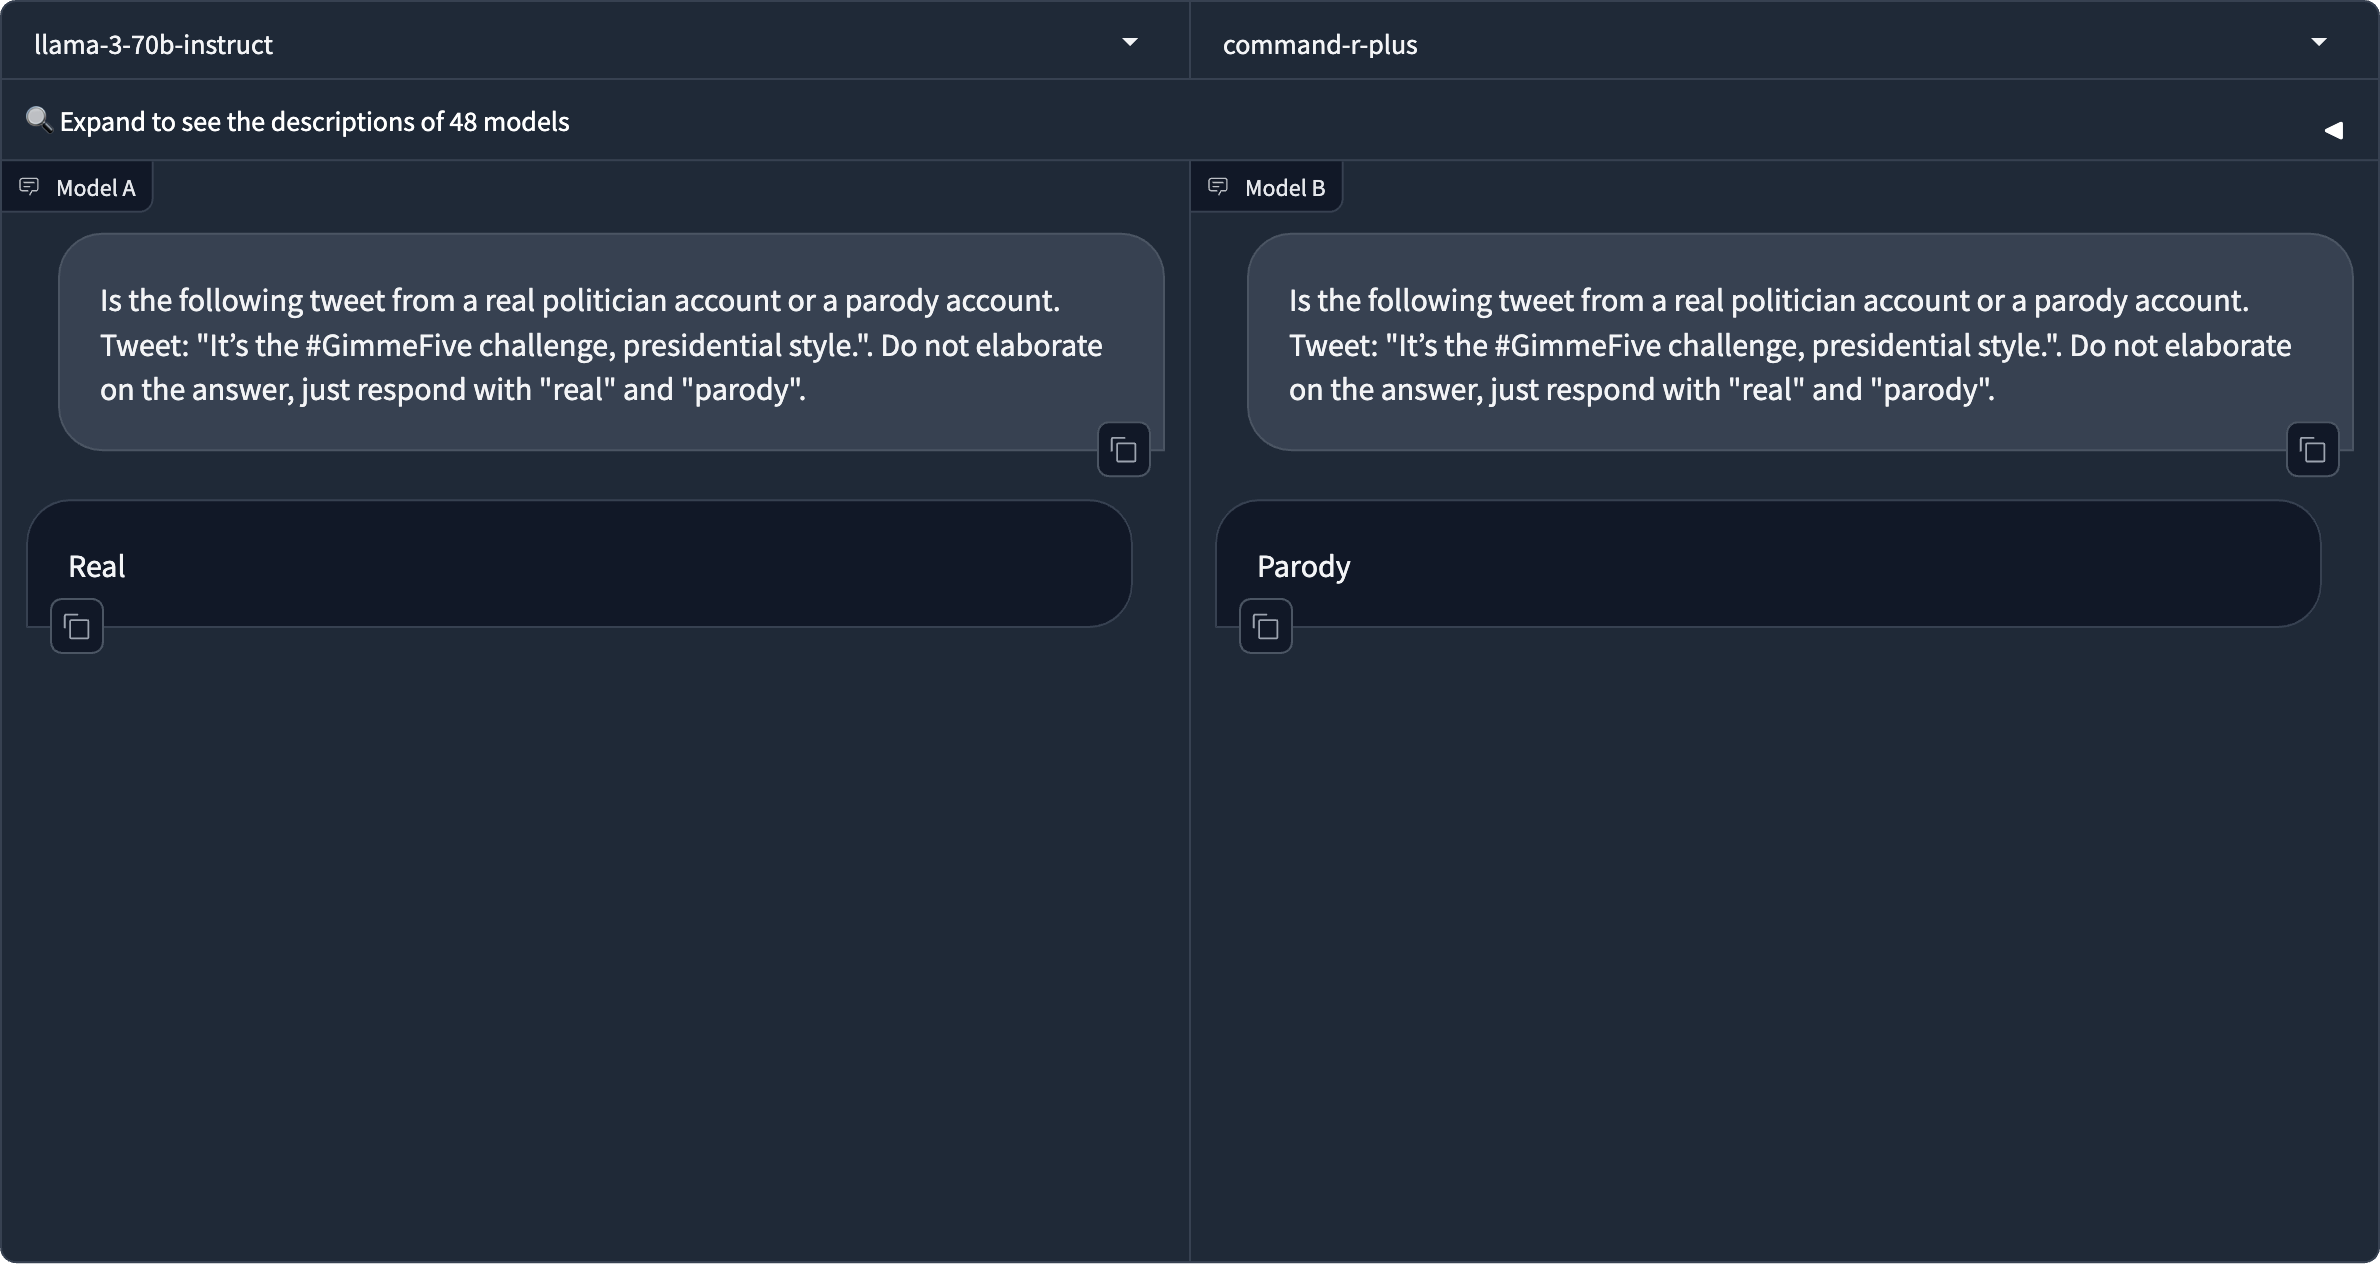
\includegraphics[width=\linewidth]{Assignment_3/Report/Figures/template-A-tweet-1.png}
    \caption{Template A on Tweet 1}
    \label{fig:A1}
\end{figure}

\begin{figure}
    \centering
    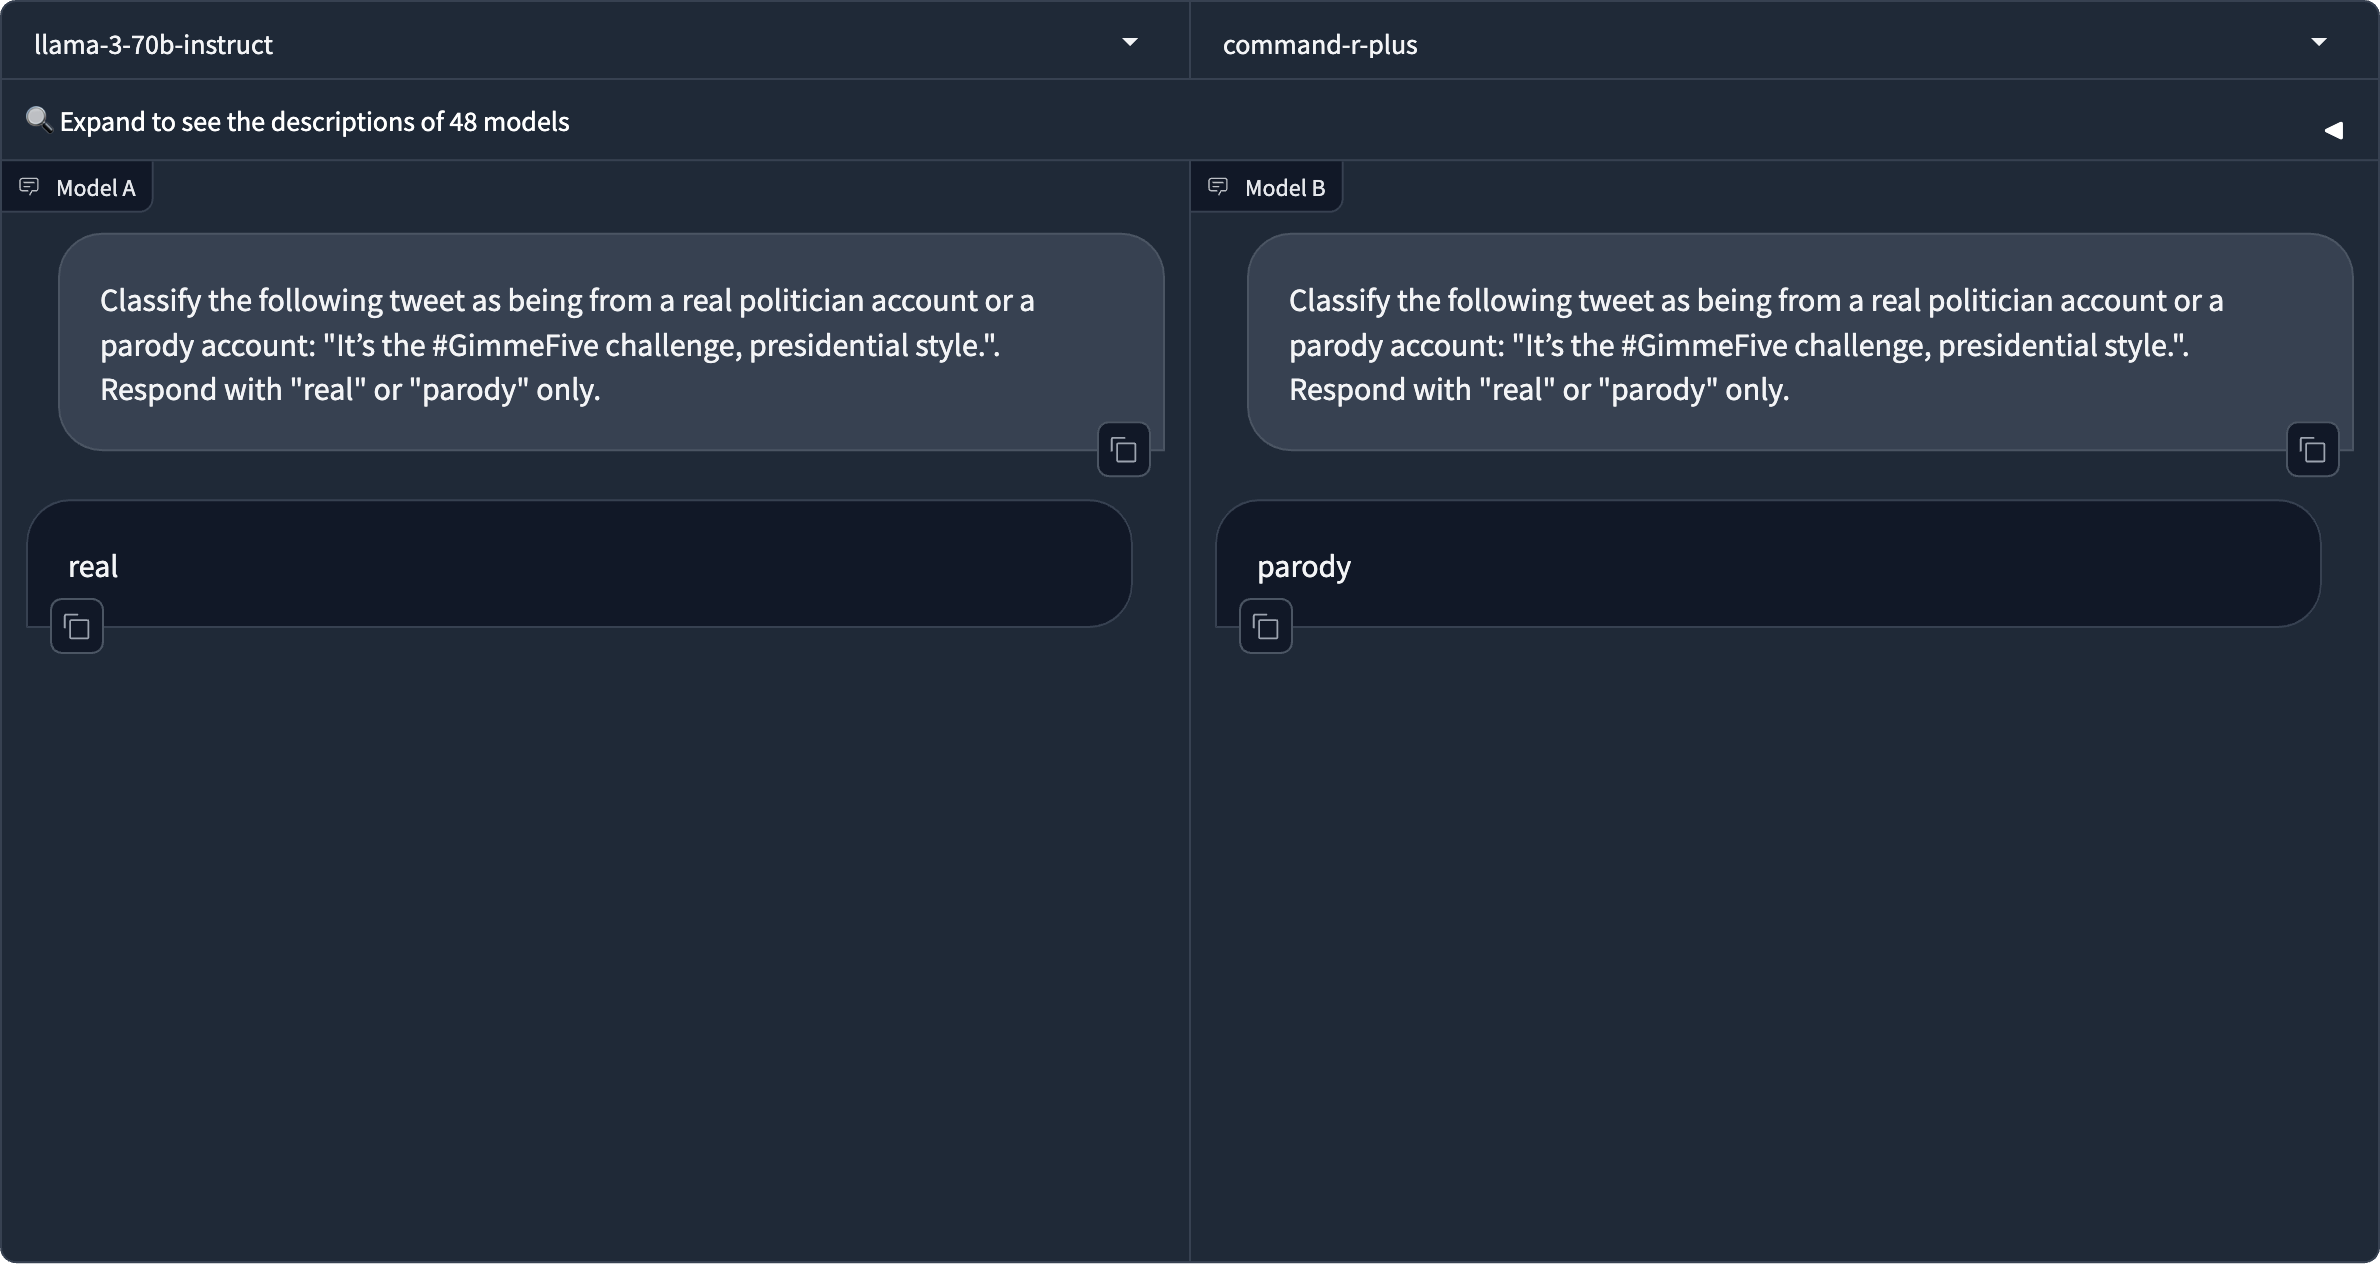
\includegraphics[width=\linewidth]{Assignment_3/Report/Figures/template-B-tweet-1.png}
    \caption{Template B on Tweet 1}
    \label{fig:B1}
\end{figure}

\begin{figure}
    \centering
    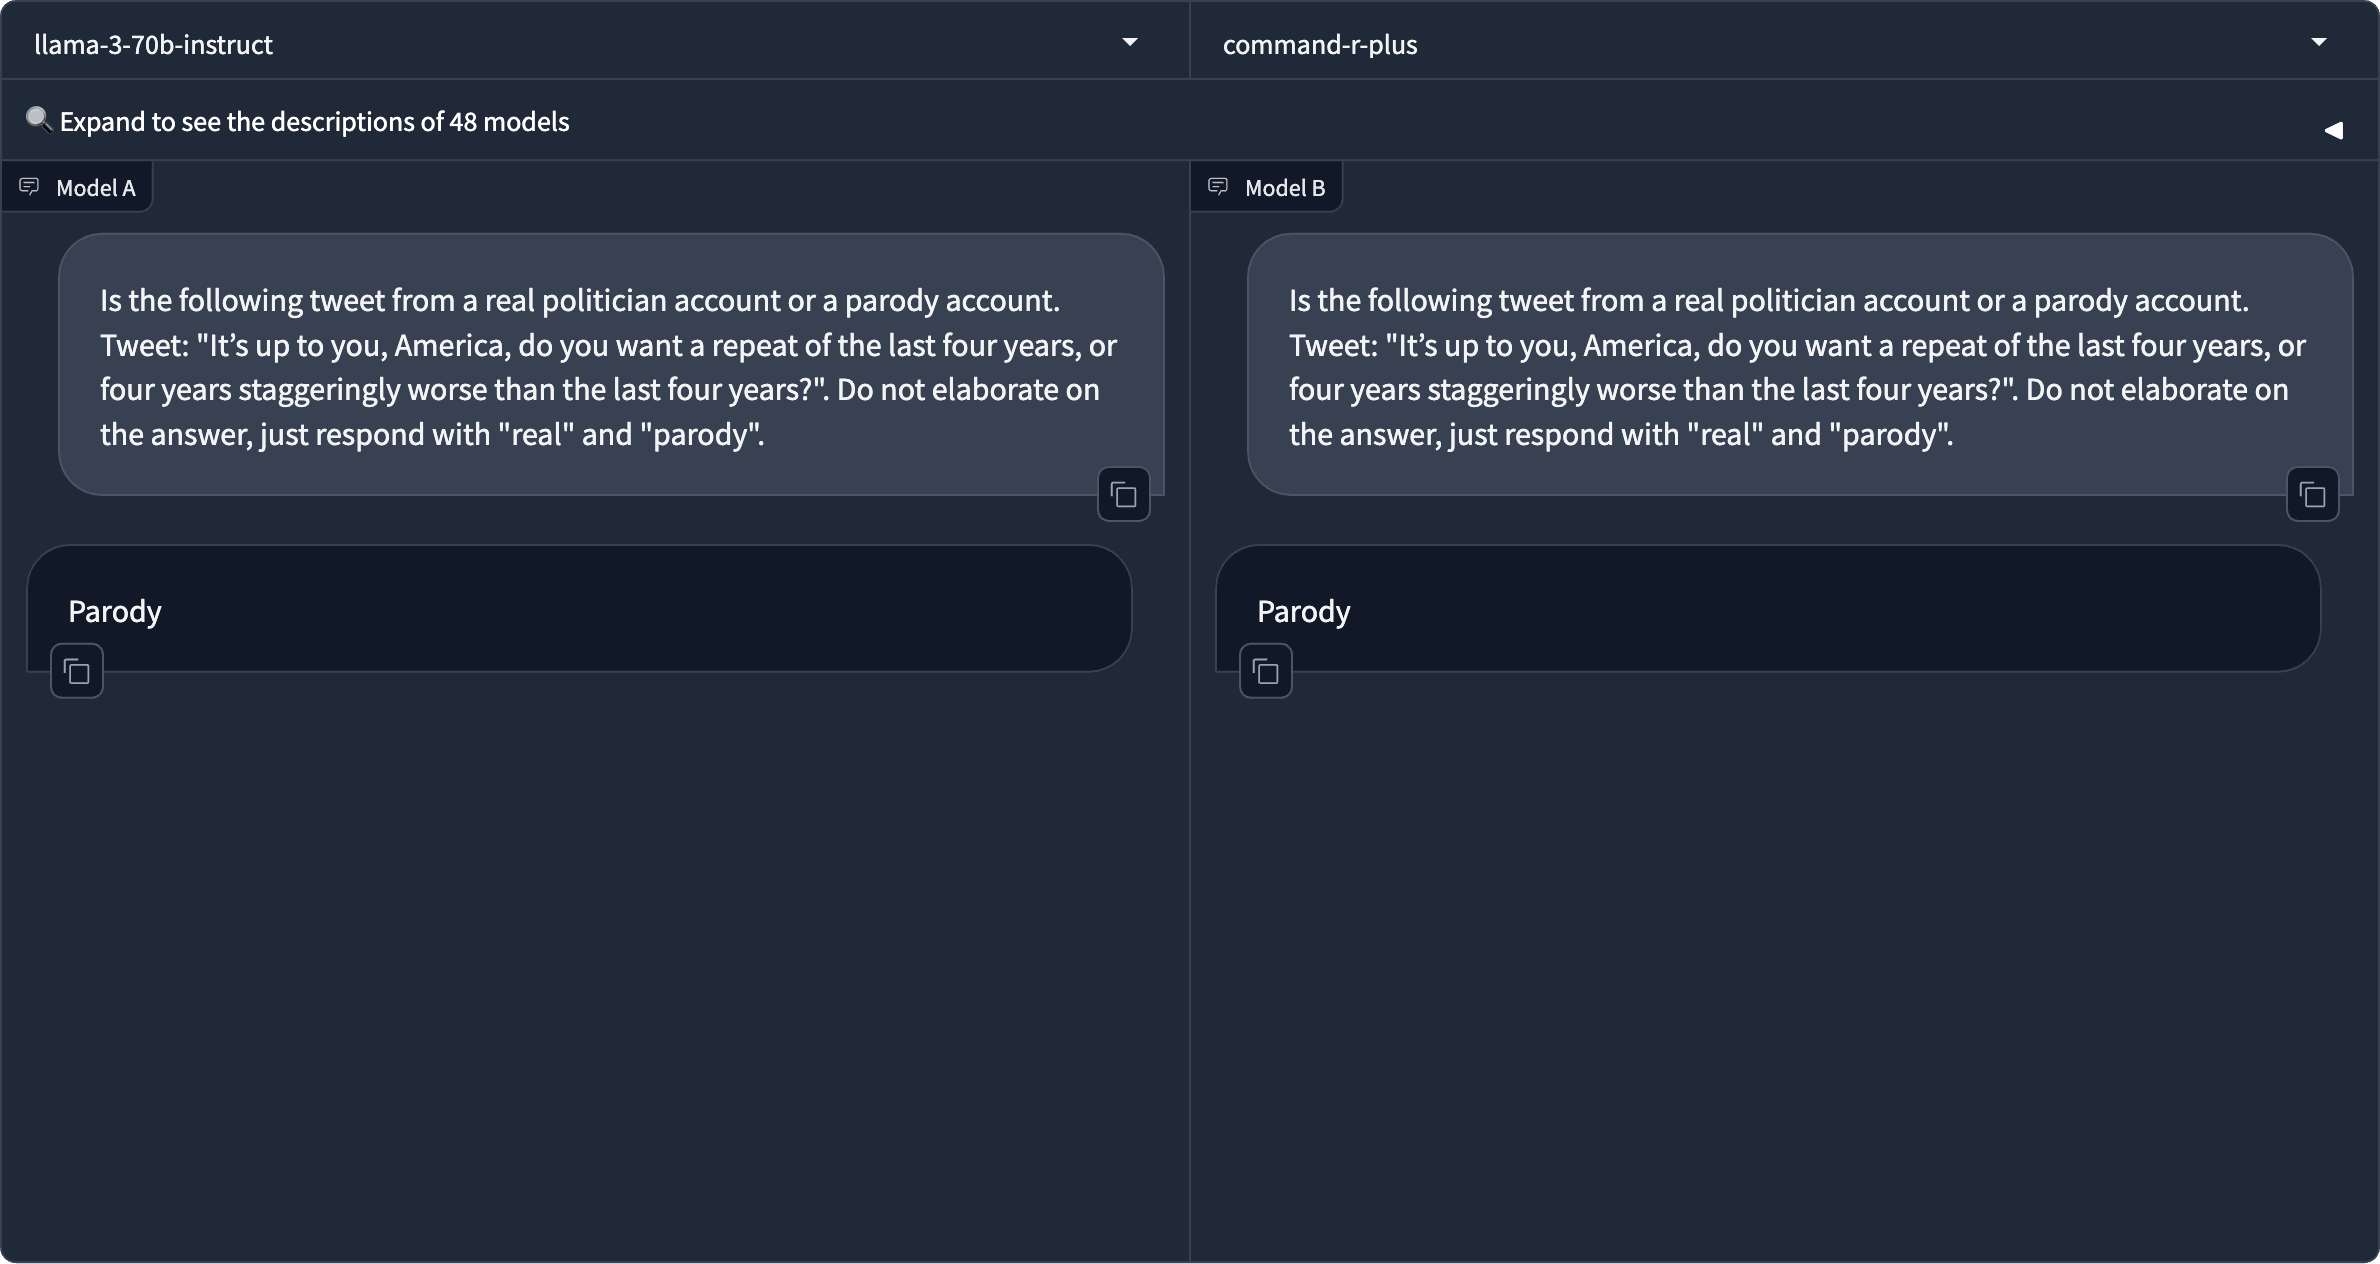
\includegraphics[width=\linewidth]{Assignment_3/Report/Figures/template-A-tweet-2.png}
    \caption{Template A on Tweet 2}
    \label{fig:A2}
\end{figure}

\begin{figure}
    \centering
    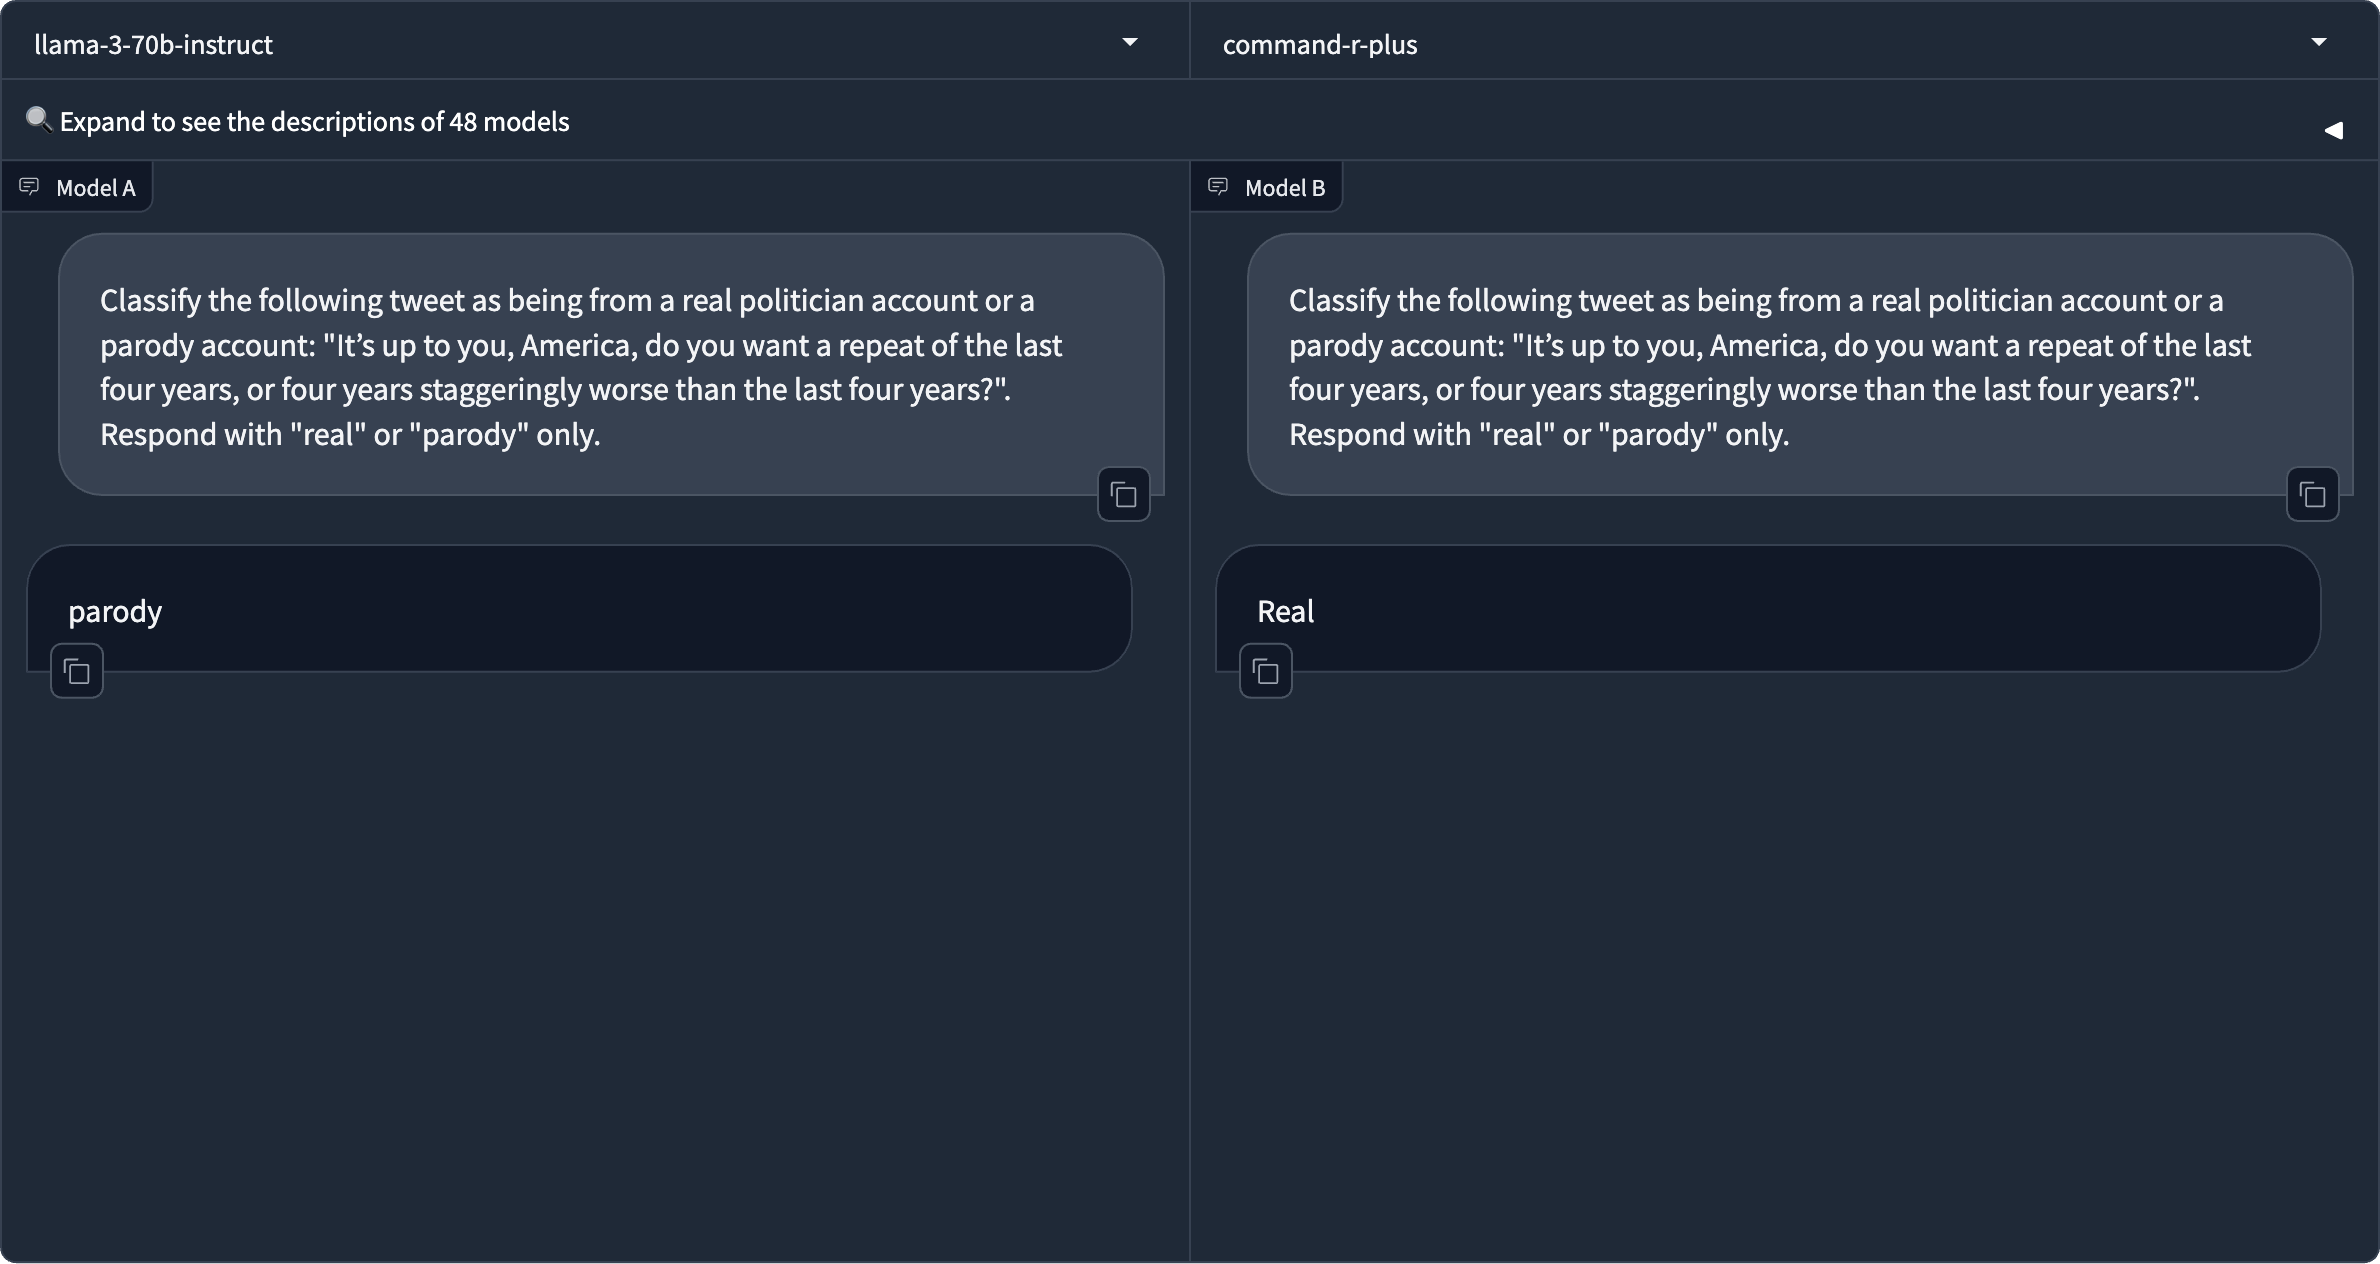
\includegraphics[width=\linewidth]{Assignment_3/Report/Figures/template-B-tweet-2.png}
    \caption{Template B on Tweet 2}
    \label{fig:B2}
\end{figure}





% \appendix
% \section{Useful tricks}
% \begin{figure}
%   \begin{center}
%     \fbox{some figure content}
%   \end{center}
%   \caption{Every figure and table has a caption and is referred to 
%     in the text body.\label{fig:q6p1}}
% \end{figure}

% You can add code like this
% \begin{lstlisting}
% c = conv(x)
% c = torch.square(c)
% \end{lstlisting}
% and like this \lstinline{torch.sum}.


\end{document}
